\documentclass[conference, 10pt]{IEEEtran}
% \usepackage{cite}
\usepackage{amsmath, amssymb, amsfonts}
\usepackage{algorithmicx}
\usepackage{graphicx}
\usepackage{textcomp}
\usepackage{xcolor}
\usepackage{subcaption}
\usepackage{flushend}
\usepackage{booktabs}
\usepackage[inline]{enumitem}
\usepackage{nohyperref}
\usepackage{url}
\usepackage{setspace}
\usepackage[utf8]{inputenc}




\def\BibTeX{{\rm B\kern-.05em{\sc i\kern-.025em b}\kern-.08em

    T\kern-.1667em\lower.7ex\hbox{E}\kern-.125emX}}

\pagenumbering{arabic}

\begin{document}

\begin{titlepage}
    \begin{center}
        \vspace*{2cm}

        \LARGE
        \textbf{HKUST President's Cup Final Report}
        \vspace{0.5cm}

        \Huge
        \textbf{Vivian: Decentralized Global Naming and Storage System on Tangle Distributed Ledger}

        \vfill

        \Large
        Written by: \\
        \vspace{0.2cm}
        TIAN Xiangan \\
        \vspace{0.2cm}
        Student ID: 20583620 \\
        \vspace{0.2cm}
        Year of Study: 3 \\
        \vspace{1.5cm}
        Supervised by: \\

        \vspace{0.2cm}
        Prof. TSOI, Yau Chat \\
        \vspace{0.2cm}
        Department of CSE


        \vfill

        \vspace{0.8cm}

        \large
        Department of Computer Science and Engineering \\
        \vspace{0.15cm}
        School of Engineering \\
        \vspace{0.15cm}
        Hong Kong University of Science and Technology

    \end{center}
\end{titlepage}

\title{Vivian: Decentralized Global Naming and Storage System on Tangle Distributed Ledger}

\author{
    TIAN Xiangan \\
    xtianae@connect.ust.hk
    \and
    Supervisor: Prof. TSOI, Yau Chat \\
    desmond@cse.ust.hk
}

\maketitle

\thispagestyle{plain}
\pagestyle{plain}

\begin{abstract}

    With the booming of distributed ledger technology (DLT) such as blockchain, many previous IT architectures can have alternative decentralized approaches for more secure, transparent, and immutable data storage.
    In this paper, we present the design and implementation of Vivian, a new decentralized global naming and storage system based on IOTA Tangle distributed ledger for re-decentralizing the current Internet service and building decentralized applications.
    The system has no single point of failure and the nodes in the network do not need to trust each other.
    Unlike the traditional Domain name System (DNS), trust points like DNS root servers are removed and critical data bindings are secured by the distributed ledger. All the nodes in the system form a peer-to-peer (P2P) network for user quires' routing.
    The P2P network is established through peer discovery protocols such as mDNS, Kademlia DHT and peers exchange data and achieve eventual consistency via Gossip protocol.
    We also provide a decentralized storage system which can hold user data securely without the control of central trust parties or revealing information to storage providers.
    By using IOTA Tangle, a directed-acyclic-graph (DAG) distributed ledger, the system inherits its scalable, lightweight, and feeless characteristics and most IoT devices have enough computational power to sign and send transactions.
    This extends the usage of Vivian to Internet-of-Thing (IoT) services for decentralizing IoT networks and enhancing IoT data security and privacy.

\end{abstract}

\section{Introduction}
\label{sec:introduction}

A distributed ledger is a type of distributed database that assumes the presence of nodes with malicious intentions.
A distributed ledger comprises a ledger's multiple replications in which data can only bye appended or read.
\section{Background}
\label{sec:background}

\subsection{Blockchain and Tangle (DAG)}
Blockchain DLT became widely known in 2009 with the launch of Bitcoin network.
Participants in the network can validate and verify the transactions independently, without relying on central trust parties.
Blockchain is usually maintained and managed by a distributed group of participants independently.
This along with its cryptographic mechanisms ensures the data recorded on the ledger immutable \cite{Yaga2018BlockchainTO}.
The structure of a traditional blockchain can be simplified as a singly linked list\footnote{Singly linked list: linked list which is unidirectional and can only be traversed in one direction.},
you can traverse from the latest block to the Genesis block\footnote{Genesis block: the first block of a blockchain. It is a special case as it does not reference a previous block.} (as shown in figure~\ref{fig:blockchain_structure}).
Transactions are hashed in a Merkle Tree \cite{merkle1980protocols} for saving storage space and simplifying transaction validation.


\begin{figure}[h]
    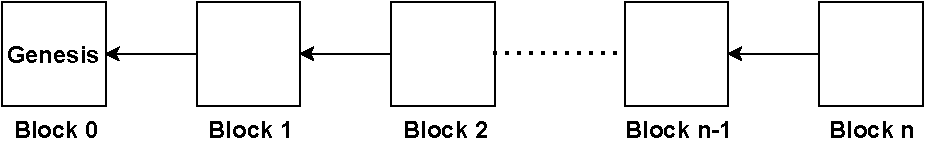
\includegraphics[width=0.45\textwidth,trim={-2cm -1cm 0 -1cm},clip]{figs/blockchain_structure.pdf}
    \caption{Blockchain structure}
    \label{fig:blockchain_structure}
\end{figure}

\begin{figure*}[t]
    \centering
    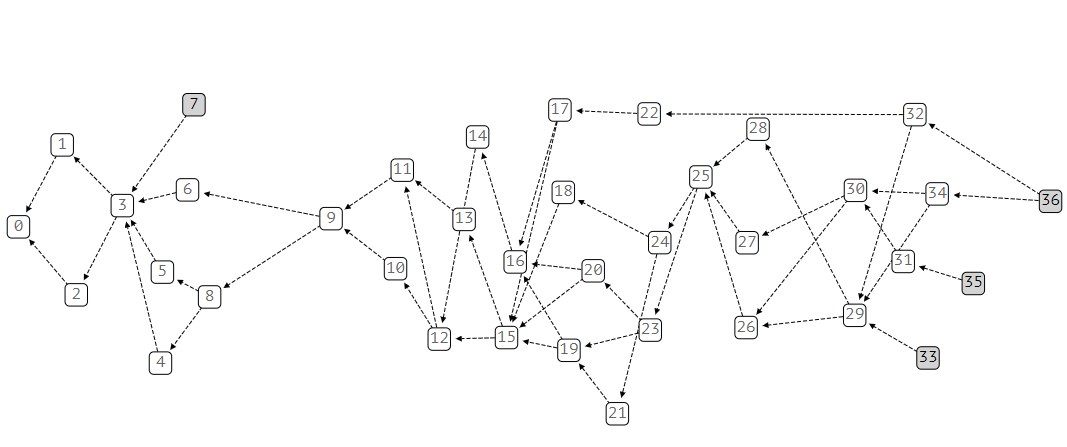
\includegraphics[width=\textwidth,trim={-1cm 0 0 2cm},clip]{figs/tangle_structure.png}
    \caption{Tangle directed-acyclic-graph structure. Shaded vertices represent tips (new transactions attaching to Tangle). The very first transaction, denoted as 0-th vertex, is the genesis transaction. It gave the total supply of IOTA tokens to one address.}
    \label{fig:tangle_structure}
\end{figure*}

In the original Bitcoin whitepaper \cite{nakamoto2008peer}, Satoshi Nakamoto has listed the procedures for handling the transactions and record them on the blockchain ledger.
All the nodes listen to the transactions broadcast to the network and each node collects new transactions for generating a new block.
Then each node will do proof-of-work and broadcast the block to the network once it finds the solution for other nodes' validation.
However, in the real case, almost all the transaction wrapping and PoW are finished by specific miners in the network. Miners also require transaction fees for the reward of doing these.
The increasing PoW complexity makes it nearly impossible to gain profit from mining Bitcoin with general PC hardware. Instead, dedicated miners have to use the equipments like ASIC\footnote{ASIC: application-specific integrated circuit. It is the integrated circuit designed for a specific use case. Bitcoin ASIC chip can only handle computing tasks for Bitcoin mining, and cannot be used for any other tasks.} specifically to the mining algorithms.
It is a potential hazard that the blockchain network will be centralized and controlled by the parties that own most of the "mining rigs". In addition, blockchains relying on PoW are consuming massive energy \cite{sedlmeir2020energy}. According to CBECI\footnote{CBECI: Cambridge Bitcoin Electricity Consumption Index. Website: https://cbeci.org/}, Bitcoin network consumes approximately 130.51 TWh electricity per year, which is far more than the annual electricity consumption of some countries like Ukraine and Argentina. Carbon dioxide emissions caused by these PoW blockchains will cause environmental issues like global warming.


Transaction throughput and transaction confirmation latency are the two most critical performance issues about blockchain technology \cite{zhou2020solutions}.
Transactions can only be recorded on the blockchain in sequence due to its linear structure. Also, the limitation of the size of each block makes it struggling to handle the enormous volume of transactions nowadays.
Blockchains including Bitcoin and Ethereum are facing problems like low TPS and bad scalability which results in transaction backlog and high transaction fees.
To tackle these issues, people have put forward many alternative solutions such as side-chain, cross-chain, improved consensus, sharding, DAG, etc.
IOTA Tangle is a new type of DLT addressing solving the problems above for IoT services. It has the following advantages comparing with traditional blockchain technologies:

\begin{enumerate}
    \item \textbf{High scalability.} Directed-acyclic-graph structured Tangle ledger enables its high scalability. Serguei Popov has analyzed the performances of the system under two different regimes: low load and high load in the article \textit{The Tangle} \cite{popov2018tangle} In high load regime when more new tips\footnote{Tip: every new (unconfirmed) transaction is known as a tip.} are attached to Tangle, the typical time of a tip being approved is reduced.
          So the larger the scale of the network, the more efficient it will be.
    \item \textbf{Feeless \& Environmentally Friendly.} In a DLT network like Bitcoin, we need to pay transaction fees to the miners for rewarding them wrapping our transactions to the block and conducting PoW computations. Transaction fees are considered part of the incentive for nodes to support the network. In IOTA Tangle, however, PoW consensus and miners are removed \cite{popov2019iota}. So it is more economical and environmentally Friendly to use Tangle for sending transactions.
    \item \textbf{Quantum Computation Resistance.} IOTA Tangle uses post-quantum cryptography for securing data on the ledger \cite{tennant2017improving}. For instance, IOTA uses Winternitz One-Time Signature (WOTS), which is promising to be resistant to quantum computers \cite{buchmann2008post} as a signature scheme protocol.
    \item \textbf{Lightweight.} IOTA node applications like GoHornet\footnote{GoHornet: IOTA full node software built in Go. Github source code: https://github.com/gohornet/hornet} is lightweight and can be easily installed and run on low-end devices such as Raspberry Pi 4.
\end{enumerate}

These characteristics are very crucial for IoT applications and favorable for critical data binding and sharing of Vivian.


\subsection{Decentralized Naming System}
Before distributed ledger technology came into being, building a decentralized naming system was considered almost impossible \cite{swartz_2011}. To build a system like it, three properties have to be satisfied:

\begin{enumerate}
    \item \textbf{Human-meaningful.} The names the system provides should be meaningful and easy to memorize, e.g. bitcoin.org. And hash values like \texttt{764569e58f53} are obviously not meaningful and hard for humans to memorize.
    \item \textbf{Secure.} The names should return the correct binding values. Damage caused by malicious entities should be as low  as possible.
    \item \textbf{Decentralized.} No central authority controls the system. Names can be chosen by users at the edge of the network rather than representative central parties.
\end{enumerate}

The challenge is that, with traditional approaches, a naming system can satisfy some of the properties, but not all three of them at the same time \cite{wilcox2001names}. This trilemma is called Zooko's triangle \cite{swartz_2011} (very similar to CAP theorem\footnote{CAP theorem: it is impossible for a distributed data store to provide, Consistency, Availability and Partition tolerance, all of the three guarantees at the same time.} in distributed system design).
Besides, the system should also ensure the uniqueness of the names, which means two different users cannot create and use the same name \cite{ali2017blockstack}.
Domain Name System in the current Internet is human-meaningful and secure, but not decentralized. Public keys are secure and decentralized, but not human-meaningful.
Zooko's Triangle has been squared by distributed ledger technology \cite{swartz_2011} and Namecoin was the first implementation to build a decentralized naming system over blockchain DL.

\begin{figure}[h]
    \centering
    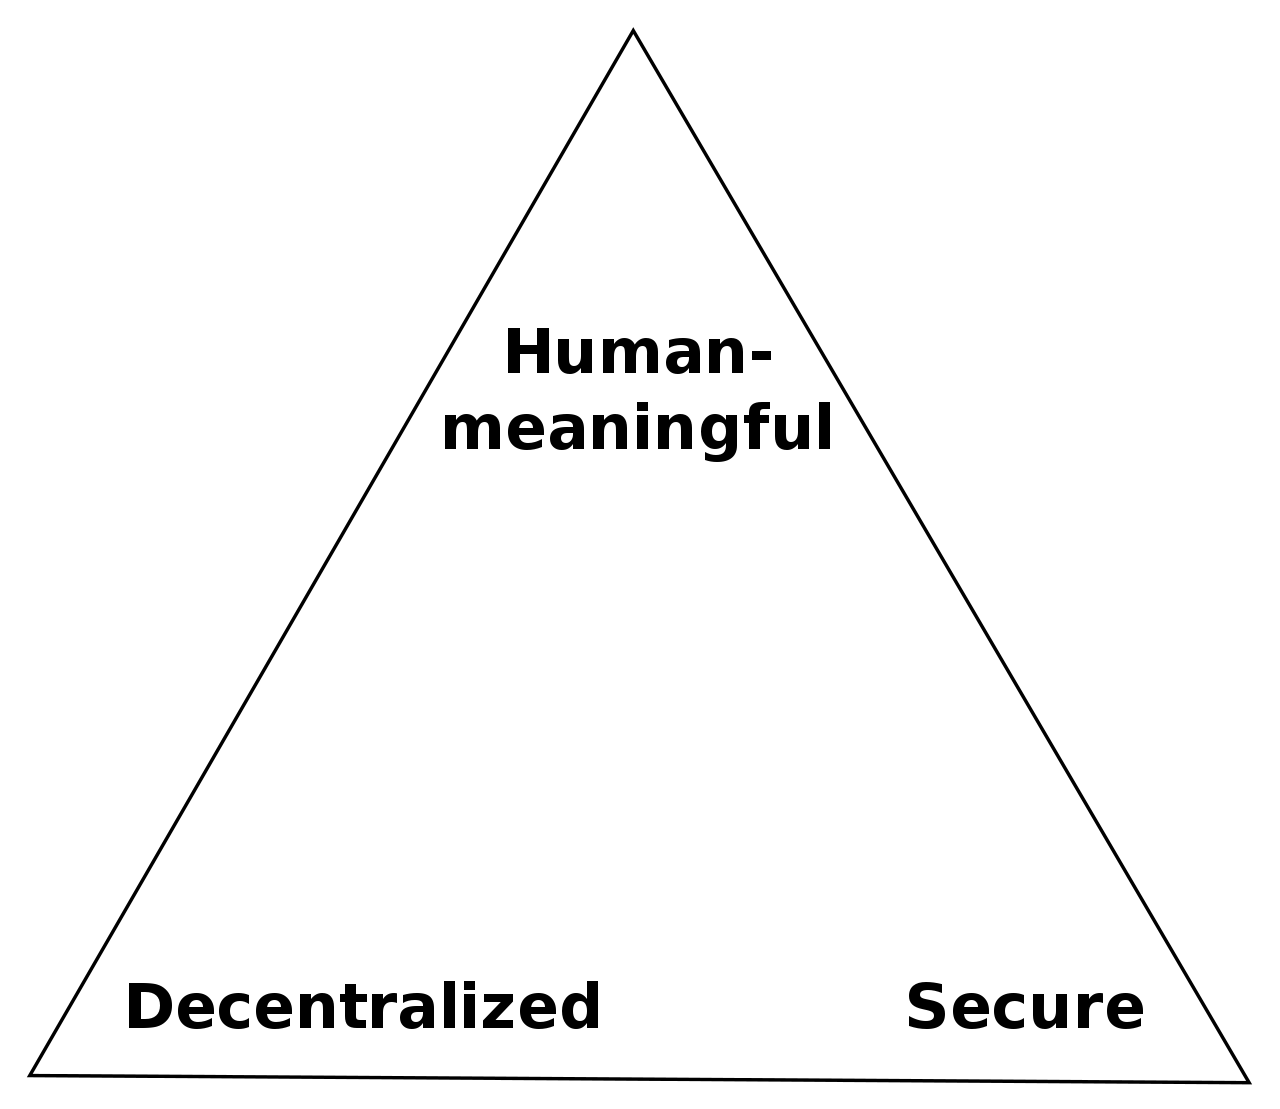
\includegraphics[width=0.2\textwidth,trim={0 0 0 0},clip]{figs/zooko_triangle.png}
    \caption{Zooko's Triangle}
    \label{fig:zooko_triangle}
\end{figure}

Blockstack is a decentralized public key infrastructure (PKI) service built on Bitcoin for building a decentralized Internet \cite{ali2017blockstack}.
The implementation of its naming system is based on the definition of a state machine and rules for state transitions on its virtualchains \cite{nelson2016extending, ali2016blockstack}.
In the design of Vivian's naming system, we referenced the ideas from Blockstack and Namecoin. 

\subsection{P2P Network}

In conclusion, peer-to-peer (P2P) networks are distributed networks in which participants provide service and content that can be accessed by other peers directly without passing through intermediate entities by shared hardware resources \cite{990434}. In a P2P network, all the peers are equally privileged, equipotent nodes that forming the network \cite{nemat2011taking}. Unlike the client-server model, a peer plays the roles of suppliers and consumers of the sources at the same time.

\section{System Design}
\label{sec:design}

\subsection{Overview}
In designing Vivian, we want the system to achieve the following properties:

\begin{itemize}
    \item \textbf{Decentralized Naming and Look-up.} End-users can register for and bind values to human-meaningful names and look up the values of names without relying on the trust of central authorities.
    \item \textbf{Decentralized and Secure Storage.} End-users can store their data in a decentralized manner. Besides, users can control the access rights of their data.
    \item  \textbf{IoT Device Supported.} The whole process like registering a name, looking up a name, and file handling should not be energy-hungry or hardware resource hungry.
          They can be accomplished by devices with limited hardware resources such as Raspberry Pi.
\end{itemize}

The overall architecture of Vivian can be divided into three layers: \textbf{Tangle DL layer, Peer Network layer, and Storage layer}.
Tangle distributed ledger is used as storage intermediate of critical data binding and for consensus of the order of the system operations.
Nodes in the peer network layer are equally privileged, equipotent peers which perform the live listening to transactions on Tangle, parsing the operations, storing naming key-value pairs, and routing for users to find the information of the names.
Storage layer is an alternative layer for users to store the name pointing data. Overview of the architecture is shown in Fig~\ref{fig:vivian_architecture}.

\begin{figure}[h]
    \centering
    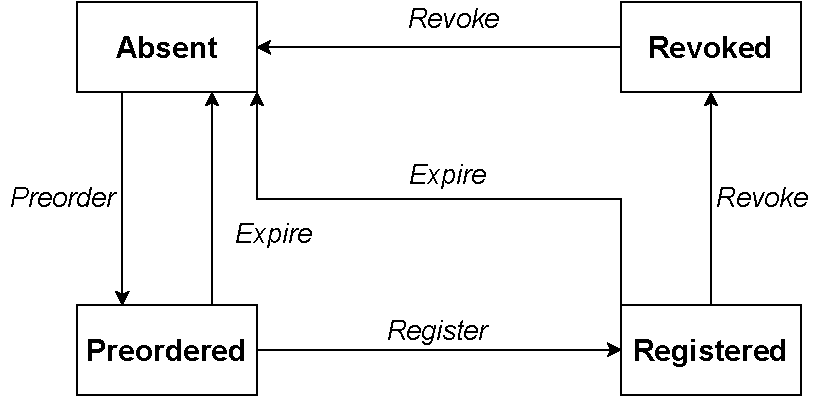
\includegraphics[width=0.4\textwidth,trim={0 0 0 0},clip]{figs/name_state_transition.pdf}
    \caption{Name state transitions}
    \label{fig:name_state_transition}
\end{figure}

\subsection{Naming System}
The design of the naming system is inspired by the implementation of Namecoin \cite{kalodner2015empirical} and BNS of Blockstack \cite{ali2017blockstack, ali2016blockstack}.
Names are owned by the cryptographic public addresses and the corresponding seed which generates the address of IOTA. In IOTA, addresses are generated by the user's private seed with Kerl Hash Function \cite{Baek2019IOTAAC}. As shown in Fig~\ref{fig:name_state_transition}, operations in the naming system perform the state transitions of names.
Each name has four states: \textbf{absent, preordered, registered, and revoked}. And \textbf{preorder, register, revoke, and expire} operations transit the state of the name into one another. In addition, as a registered name, \textbf{renew, update, and transfer} operations can be performed for changing its binding value.

To claim a name, a user needs to first preorder the target name and then register it. Preorder operation is for users to indicate interest in the name. The operation sends a transaction with the message containing the hash commitment of desired name rather than plain text. The reason for sending hash commitment is to prevent front-running \cite{kalodner2015empirical}, e.g., if a name is revealed to the public, an attacker can race the user for claiming it \cite{ali2016blockstack}.
The preorder operation also acts as a signal for the nodes in the peer network to start the preprocessing of a name registration.
After preorder, the user can send the register operation for providing the name he/she wants to claim, the transaction hash of the previous preorder transition, the keys for decrypting the hash commitment, and the value for name binding.
The first user who finishes both preorder and register operation successfully will grant ownership of the name.
And any preorder operations performed by the other users will be invalid. In Namecoin's implementation, \texttt{NAME\_NEW} and \texttt{NAME\_FIRSTUPDATE} operations are equivalent to the preorder and register operations in Vivian.
For the effectiveness of \texttt{NAME\_NEW} and front-running prevention. The gap between \texttt{NAME\_NEW} and \texttt{NAME\_FIRSTUPDATE} transactions should be no less than 11 blocks \cite{kalodner2015empirical}. In Vivian, we count the gap by timestamps between two transactions. The details will be described in Section~\ref{sec:implementation}.

After a name becomes registered, the owner can send an update transaction for updating the name-value binding. He/She can also transfer the name to others by sending the transfer transaction to change the address that signs subsequent transactions. Revoke operation is used for disabling any further operations on the name. After that, the name-binding value cannot be changed until expiration.

A name in Vivian is not permanent and has a certain time for expiration. In Namecoin, the original period for a name to expire is 36,000 blocks (around 250 days).
It means if a name hasn't been mentioned in \texttt{NAME\_UPDATE} or \texttt{NAME\_FIRSTUPDATE} in 36,000 blocks, it becomes absent again \cite{kalodner2015empirical}.
In Vivian, the expiration time is counted by the timestamp of the register transaction. Besides, users can send the transaction for renewing their names before expiration.

By using Tangle DL, most IoT devices have enough computational power to sign and send the transactions for naming operations \footnotetext{For more detail: \url{https://docs.iota.org/docs/iot/0.1/introduction/overview}}.

\subsection{Peer Network}
Nodes in the peer network form a routing layer for users to find the binding value of names.
Every node will consistently listen to all the transactions on IOTA Tangle and filter the transactions that relate to Vivian naming operations.
Then it parses the transaction and updates the name key-value bindings in its local database.
In the local database, basically, a node only needs to record the registered names and the address and hash of the latest transactions that modify a name binding value. A node can also cache the binding values of the names.
When a node discovers a change of a name, e.g., a new name has been registered or a name's binding value has changed, it will record the change to the change list and periodically fan-out the change list to other k random neighbors via Gossip protocol \cite{10.1145/41840.41841}.
If a node receives the change list from another node, it will compare the changes with items in the local database. If a difference is found, it will then choose the records with the latest transaction (through timestamp comparison) and validate it by checking the transaction on Tangle DL. If the change is validated, the node then updates the change to its local database and appends the change to its change list.
If a user wants to get the binding value of a name, he/she can connect to one or more nodes in the network and query for name information. The node should return the name, the recorded transaction hash, and cached binding value (for fast access if available). The end-user does not need to trust the node as the data integrity can be validated on Tangle DL via transaction hash.
The whole peer network is established via Kademlia Distributed Hash Table (Kad-DHT) \cite{maymounkov2002kademlia} and new nodes can join the network. Once a new node joins the network, it can construct all the naming information by iterate all the transactions on Tangle DL.

\begin{figure}[h]
    \centering
    \begin{subfigure}[t]{0.45\textwidth}
        \centering
        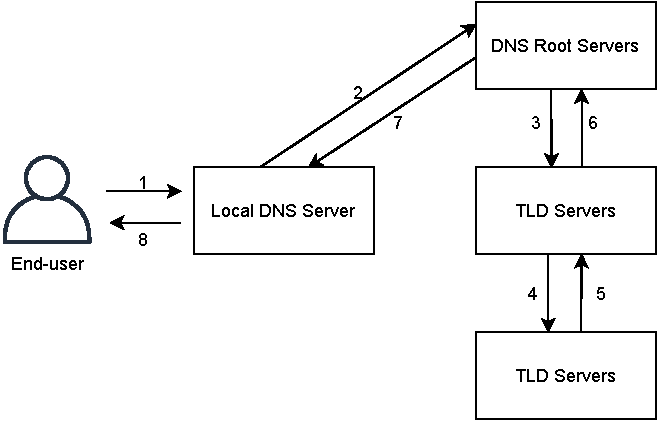
\includegraphics[width=\textwidth,trim={0 0 0 -0.5cm}]{figs/dns_routing.pdf}
        \centering
        \caption{DNS}
    \end{subfigure}
    \centering
    \begin{subfigure}[b]{0.45\textwidth}
        \centering
        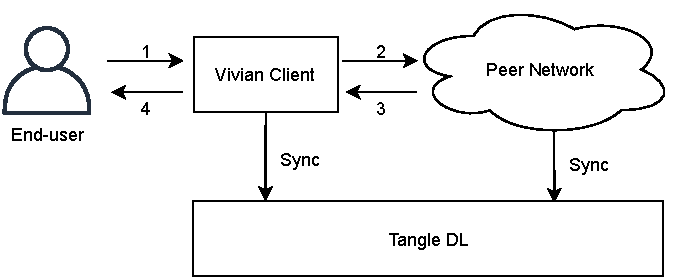
\includegraphics[width=\textwidth,trim={0 0 0 -0.5cm}]{figs/vivian_routing.pdf}
        \centering
        \caption{Vivian}
    \end{subfigure}
    \caption{Comparison of DNS and Vivian queries}
    \label{fig:query_compare}
\end{figure}

Through peer network routing layer, users can query the value of a name without relying on the trust of third parties.

\subsection{Storage System}
There is no restriction on what type of data a name should map to. The storage layer provides an alternative way for binding large files to the names.
Due to the data size limitation of Tangle transaction and complexity for checking the message content of the transaction, actual data are stored on the storage layer instead of Tangle DL.
Users can choose to use InterPlanetary File System (IPFS) \cite{benet2014ipfs}, a P2P decentralized file system, to save their files or traditional storage backends such as Amazon S3, Azure Blob, Google Cloud, etc.
The design goals are to let the users own the access right of their data, users do not need to trust the storage layer and can verify the data integrity, and the other third parties like the storage providers cannot tamper with the data.
Possible implementations will be discussed in Section~\ref{sec:implementation}.

\begin{figure*}[h]
    \centering
    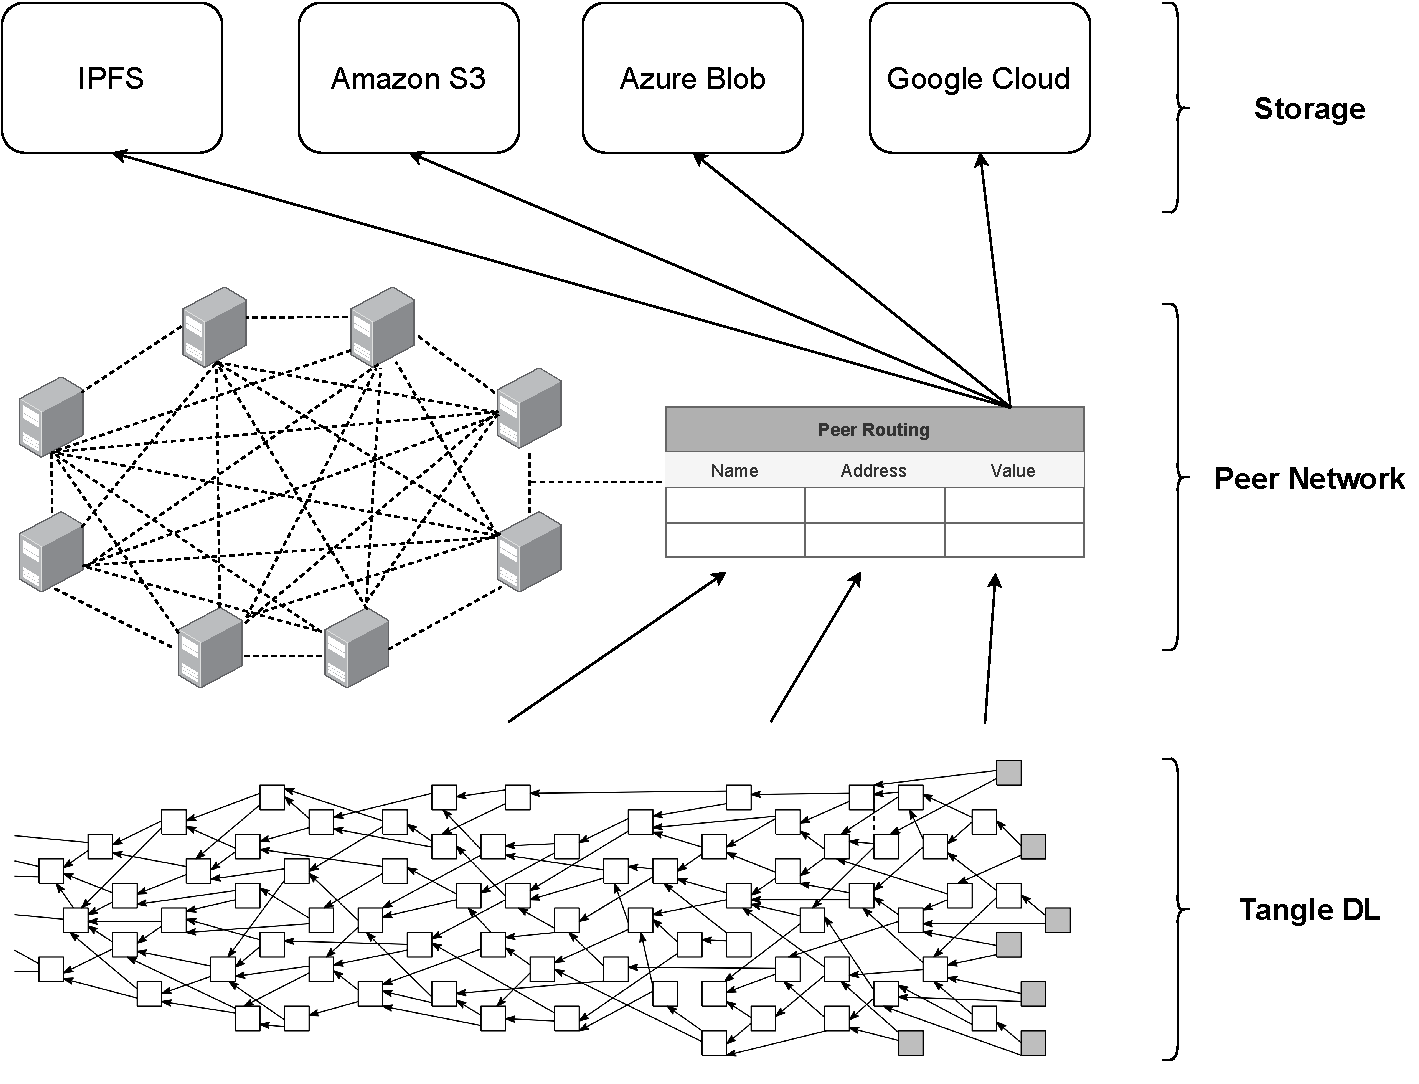
\includegraphics[width=0.8\textwidth,trim={0 0 0 0},clip]{figs/vivian_architecture.pdf}
    \caption{Vivian Architecture}
    \label{fig:vivian_architecture}
\end{figure*}
\section{Implementation}
\label{sec:implementation}

In this section, we introduce some existing implementations of Vivian and some other potential implementations for the planned features.

\subsection{Software \& Dependencies}

The whole project is currently developed in Golang v1.16\footnotetext{Golang website: https://golang.org/}.
And the platform is divided into two parts: the node software, \textit{vivian-node}, and the client software, \textit{vivian-client}.
In the future, there will be another version of the node software, which runs as a plugin of GoHornet, IOTA's node software built in Golang.
The advantage of this version is for direct access to a network instead of connecting to and trust other parties' nodes.

\subsubsection{Node Software} It sets up a node in the peer network layer. These nodes form and help to maintain a decentralized P2P network which let users to find naming information.
Each node keeps track of the naming key-value bindings by listening to the live transactions on Tangle DL, filtering naming transactions, parsing transactions, and update related key-value information on local database.
For listening live transactions, the current implementation subscribes ``tx" (incoming new transactions) and ``sn" (confirmed new transactions) topics of a IOTA node's ZMQ\footnote{ZMQ: ZeroMQ, an asynchronous messaging library for distributed or concurrent applications by providing a message queue.} port.
In the plugin version, Vivian node is also an IOTA node, so that live transactions can be retrieved from local database directly.
Besides, the node software is also responsible for handling user requests such as checking whether his/her naming operations are successful and , getting the name binding values, checking the Availability of a name, etc.

\subsubsection{Client Software} It provides a user interface (currently CLI) for sending name operation transactions and requests to peer network nodes.
When initializing the client software, it creates an IOTA seed and encrypt it with password or load a seed from a local encrypted file.
Then users can use the seed to generate public addresses and send transactions for name registration, update, revoke, etc.
The client software can also connect to the nodes in peer network layer, for finding the name binding value, and validating name operations.

\subsubsection{Dependencies} In operating Vivian, we need to do a lot of work related to key-value pairs, and information is stored in \textit{BadgerDB}\footnote{BadgerDB: an embeddable, persistent and fast key-value (KV) database written in pure Go. Github repository: https://github.com/dgraph-io/badger}.
We use libraries in \textit{iota.go}\footnote{iota.go: official Go client library for interacting with the Tangle. Github repository: \url{https://github.com/iotaledger/iota.go}} for handling transactions on Tangle.
We use functions in \textit{go-libp2p}\footnote{go-libp2p: implementation of the libp2p networking stack in Golang. Github repository: \url{https://github.com/libp2p/go-libp2p}} for peer discovery and peer Communication in the P2P network.
Communication messages are serialized by \textit{Protocol Buffers}\footnote{Protocol Buffers (Protobuf):  a method of serializing structured data. Its performance is even better than JSON.} for better performance.

\subsection{Naming Operations}
In this subsection, we introduce how naming operation information is recorded via transactions on Tangle. And taking name registration as an example, for having an overview of how the naming operations are executed.

\subsubsection{Name Operation Transactions} There are two types of transactions in IOTA Tangle: zero-value transaction and value transaction. And currently we use zero-transaction format for name operation transactions.
Zero-value transactions are barely transactions with value 0 in the \texttt{value} field.
Data of transactions are encoded in trytes\footnote{Tryte: a concept in ternary numeral system similar to byte in binary numeral system. See details on: \url{https://docs.iota.org/docs/getting-started/0.1/introduction/ternary}}.
Each transaction consists of 2,673 tryte-encoded characters. After decoding the trytes, we can obtain the a list of data fields of a transaction. The fields related to naming operations are:

\begin{itemize}
    \item \texttt{hash}: 81-tryte string. It is the transaction hash derived from the values of every transaction field and contains part of the proof-of-work. We can use transaction hash to track and validate the information of a transaction.
    \item \texttt{signatureMessageFragment}: 2,187-tryte string. It is a signature or a message, both of which may be fragmented over many transactions in a bundle.
          This field is used for saving the naming operation information, and name binding values. 2,187 trytes' size is enough for most of the use cases.
    \item \texttt{attachmentTag}: 27-tryte integer. It is user-defined tag. This field is used for accelerating the filtering of the live transactions.
          For fast selection of related transactions, users are required to set the corresponding two-character logogram for each naming operation transaction.
          And nodes in peer network layer can use tryte formats of the logograms for comparison and identifying name operation transactions without parsing \texttt{signatureMessageFragment} (see TABLE~\ref{table:tags}).
    \item \texttt{address}: 81-tryte string. It contains either the sender's or recipient's address. The address is used for justify the ownership of a name.
    \item \texttt{attachmentTimestamp}: 9-tryte integer. It is Unix epoch (milliseconds since Jan 1, 1970 after proof of work was done). The timestamp is used for counting the time of the operations, e.g. deciding if the current name is expired.
\end{itemize}

Proof-of-work in the previous description is different from the PoW consensus mechanism in Bitcoin blockchain.
Proof-of-work in IOTA is the method for preventing spamming in the network, similar to Hashcash\footnote{Hashcash: a proof-of-work system used to limit email spam and denial-of-service attacks.} in email system.

\begin{table}[h]
    \centering
    \begin{tabular}{||c c c||}
        \hline
        Operation & Two-Char Value & Tryte Value \\ [0.5ex]
        \hline\hline
        Preorder  & PO             & ZBYB        \\
        Register  & RG             & ACQB        \\
        Renew     & RN             & ACXB        \\
        Update    & UD             & DCNB        \\
        Transfer  & TF             & CCPB        \\
        Revoke    & RV             & ACEC        \\ [1ex]
        \hline
    \end{tabular}
    \caption{Tags for fast name operation identification}
    \label{table:tags}
\end{table}

\subsubsection{Name Registration} For sending each naming operation transaction, the client software needs to generate a new address by the private seed.
To register a name, the user should send name preordering first. In the current implementation, we use Pedersen Commitment \cite{pedersen1991non} for committing the name.
Client software creates and sends a zero-value transaction with tag ``PO" and the message: ``\texttt{PREORDER : \textlangle Hash Commit Value\textrangle}".
After the transaction is successfully sent, the client software will record the name, transaction hash, G, H, R value of Pedersen commitment to BadgerDB.
IOTA nodes will not receive transactions with timestamps more than 10 minutes ago, so in order to prevent front-running, we set the time gap of preorder operation and register operation to be 15 minutes.
After 15 minutes, the user can then send the transaction for name registration. Client software will send a zero-value transaction with tag ``RG", and message containing the name, G, H, R of pedersen commitment, preorder transaction hash and binding value of the name.
Nodes in the peer network layer keeps listening the live transactions on Tangle. If it detects a transaction with tag value in tryte ``ACQB" with appending 9s, it will parse this transaction and check the format of the message.
Then it use the information provided in the message field to validate name registration. Once the validation is confirmed, it records the name information on its local database and append this change to the change list.
The change will be broadcast to other nodes in the network via Gossip protocol later.

\subsection{Network}
libp2p network stack provides very powerful functionalities for establishing a distributed network.

\subsubsection{Peer Discovery}
Following procedures are implemented in peer discovery:

\begin{enumerate}
    \item \textbf{Bootstrap.} Nodes will often connect to a bootstrap node through its well-know IP address, to join the network for the first time.
    \item \textbf{mDNS.} Nodes can discover peers under the same local network through multicast DNS.
    \item \textbf{DHT Random Walk.} This process is for finding more peers in the network. First we make a random node ID in the network, and random walk is a query for finding the peer with that ID.
          We ask the peers we know whether they know the node with target ID or not.
          If they do not know, they will recommend the nodes with closer IDs (logic distance calculated by XOR). We continue this process until no closer node can be found.
\end{enumerate}

\begin{figure}[h]
    \centering
    \begin{subfigure}[t]{0.24\textwidth}
        \centering
        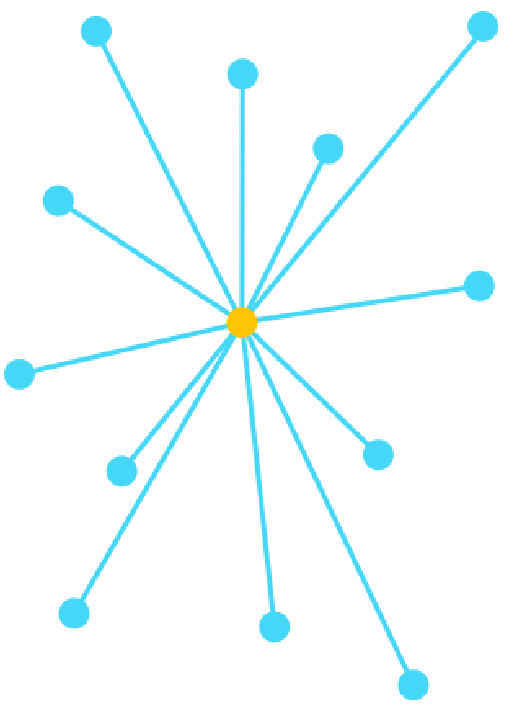
\includegraphics[width=0.4\textwidth,trim={0 0 0 0}]{figs/bootstrap_p2p.pdf}
        \centering
        \caption{Bootstrap}
    \end{subfigure}%
    \begin{subfigure}[t]{0.24\textwidth}
        \centering
        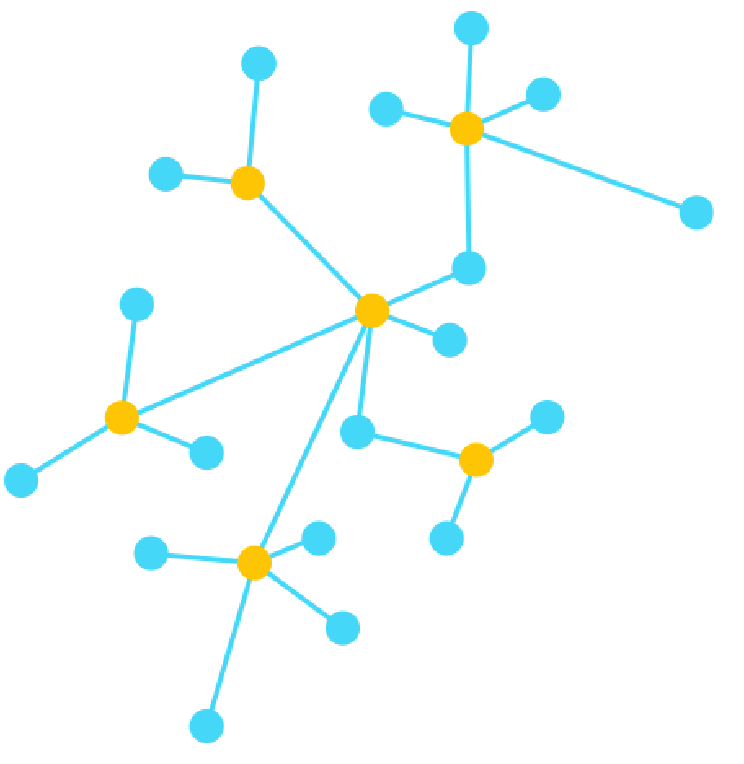
\includegraphics[width=0.5\textwidth,trim={0 0 0 0}]{figs/mdns_p2p.pdf}
        \centering
        \caption{mDNS}
    \end{subfigure}\\[1ex]
    \centering
    \begin{subfigure}[b]{0.4\textwidth}
        \centering
        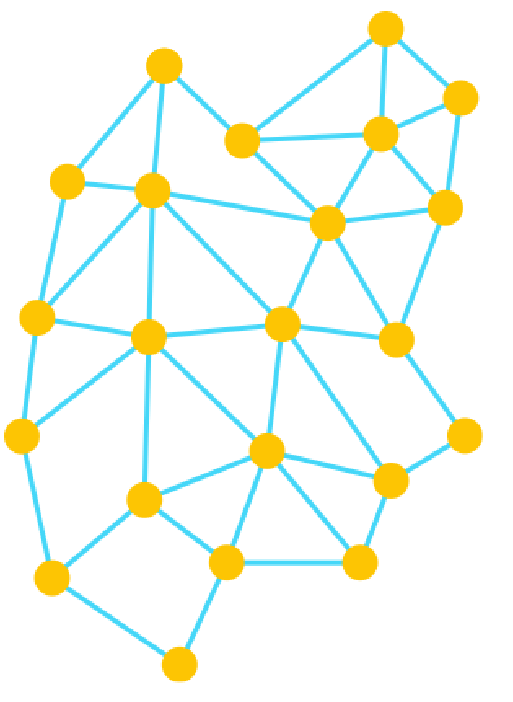
\includegraphics[width=0.25\textwidth,trim={0 0 0 0}]{figs/dht_p2p.pdf}
        \centering
        \caption{DHT Random Walk}
    \end{subfigure}
    \caption{Network structure after each peer discovery procedure}
    \label{fig:peer_discovery}
\end{figure}

\subsubsection{Peer Communication}
Vivian defines different libp2p protocols for different types of communications.
Messages are serialized via Protocol Buffers for better transmission performance.
For naming information updating among peers. We will going to implement Episub (similar to Gossip protocol) in libp2p pubsub protocols.
Considering the message redundancy issue, we plan to store the recently changed naming key-value pairs in cache for fast loop-up when handling gossip message from neighbors.

\subsection{Storage}
In this subsection we describe two potential implementations of file storage layer: via IPFS and via normal storage backends.

\subsubsection{IPFS}
IPFS is a decentralized peer-to-peer file system. When a file is uploaded to the system, it is split into many small blocks linked by a Merkle DAG.
The file and all of its blocks are given a unique hash fingerprint. The blocks of a file will be stored on different peers in the network in a distributed way.
Users can use the fingerprint of the file for content addressed searching for the file content.
The whole system is decentralized and files stored on the system are immutable. However, the fingerprint of a file is a cryptographic hash which is not human-meaningful.
Besides, traffic between nodes and content of the blocks are not encrypted and are visible to public.
In Vivian, if a user want to store his/her data via IPFS, he/she can first encrypt the file using GPG\footnote{GPG: GNU Privacy Guard. Open source alternative of Pretty Good Privacy (PGP)} and then upload to IPFS, then bind the fingerprint of the file to the name he/she owns.

\subsubsection{Normal Storage Backends}
Users can storage their data on normal storage Backends such as Amazon S3, Azure Blob and Google Cloud.
The intuitive idea is to split the file into small chunks encrypted and/or signed by user.
Then record the URI of these chunks on Tangle, and bind it to the name the user owns.
The message field of a Tangle transaction is 2,187 trytes in size and can sufficiently records a large number of URLs.
If the a single transaction is not enough to record all the URL, hierarchy tables can be implemented (similar to the idea of Bigtable by Google \cite{chang2008bigtable}).
In this way, the storage providers are only able to see the encrypted file chunks, and cannot parse the actual content of the files.
\section{Evaluation and Discussion}
\label{sec:discussion}
\section{Applications}
\label{sec:application}

Vivian is designed to be a infrastructure for reconstructing the current Internet services in a decentralized manner.
It is built on Tangle distributed ledger for a better expandability of features in Internet-of-Things Services.
To better understand how Vivian can be implemented in real-world scenarios, we list some potential use cases below:

\begin{itemize}
    \item \textbf{Decentralized Website.} Users can build and maintain their website through Vivian decentralized naming system and storage layer.
          Compared with traditional websites, decentralized websites are censorship-resistance (only the owners can censor or modify the the content of their websites),
          more robust (it is much more difficult to take them down or DDoS), and private (the owner of the decentralized websites can be anonymous).
    \item  \textbf{Identity Attachment.} Users can attach identity information such as GPG public keys, email address, cryptocurrency addresses that are not human-meaningful or easy to memorize to name they like.
    \item \textbf{Enhance IoT Scalability and Privacy.} Inferior scalability, server failure, large-scale data management, and data privacy are four of the weaknesses of the current IoT network implementation \cite{farahani2021convergence}.
          Traditionally, all the data is transmitted from a device or an object to central cloud servers where it is stored and analyzed. If the centralized server fails, the whole network is at risk of taken down.
          As more and more devices joining IoT network, scalability issues are getting worse. Also these devices are producing massive amounts of data including sensitive information, and large-scale data management and data privacy issues are becoming more severe.
          Vivian and IOTA can help to decentralize the current IoT network, and data can be stored on Tangle DL or storage layer provided by Vivian. This improves the scalability and data privacy of IoT services.
\end{itemize}


\section{Conclusion}
\label{sec:conclusion}

Current Internet services based on centralized data models have potential risk of single point of failure. 
And data storage relies on the trust of third parties such as service providers. This leads to user data integrity and privacy issues.
In this paper, we introduce Vivian, a new decentralized global naming and storage system, which is a possible solution to the problems above.
Vivian squares Zooko's Triangle trilemma and provides a decentralized naming system, that allows users to register human-meaningful names with binding information.
Its storage layer also helps users to save their files in a decentralized and secure way. 
Unlike other blockchain based decentralized naming system, Vivian uses IOTA Tangle DL for critical data binding. 
Tangle is a lightweight and highly scalable DAG distributed ledger, which allows devices with poor computing power to write and send transactions on it.
It extends Vivian's usage in IoT networks.
In addition, the system is more environmentally friendly compared with other PoW blockchain applications as it does not require miners to do Proof-of-Work computations.
We hope the design of Vivian can help inspire more innovations of DLT applications to make more impacts in different industries.


\newpage

\bibliographystyle{ieeetr}
\bibliography{main}

\end{document}